To attempt at reconstructing the truth from incomplete observations, it is generally of interest to understand the underlying statistics. Classical and quantum optics provide a comprehensive theoretical foundation to explain photon statistics. For instance, it is well understood that photons from a coherent light source follow a Poisson distribution, often referred to as shot-noise. Whereas, for chaotic (bunched) light, the variance exceeds that compared to their mean, dubbed super-Poissonian. And finally for a squeezed light source, the distribution is sub-Poissonian \cite[Chapter~5]{foxQuantumOpticsIntroduction2006}.

The same principle can be extended to photoelectron emission. For the case of emission events when photons impinge on a material, \citeauthor{mandelFluctuationsPhotonBeams1958} \cite{mandelFluctuationsPhotonBeams1958,mandelFluctuationsPhotonBeams1959} showed that the probability distribution of photoelectron counting follows the photon statistics.

In Section~\ref{sec:poisson-noise-model}, we introduced the assumption that the noise is Poisson distributed. In this chapter, we begin by formally defining a general model for counting photoelectron event data using point processes, that includes the Poisson distribution for coherent light sources and \gls{NB} distribution for \gls{SASE} \gls{FEL}. These are specifically We then test the hypothesis on data generated from a pulsed coherent light source and an \gls{FEL}

\section{Modelling Photoelectron Statistics}\label{section:photoelectron-counting-stats}
Let us start by developing an intuition for why photons exhibit stochastic behavior. Photons are the quantized form of electromagnetic light and can be thought of as discrete energy packets. The energy of a photon is given by $E = h\nu$, where $h$ is the Planck constant and $\nu$ is the frequency of the light. Due to the discrete nature of photons, it can be shown that the number of photons in a short time interval $\Delta t$ is not constant. These fluctuations are known as photon shot noise.

For a light source with a constant flux\footnote{Flux is the average number of photons passing through the cross-section of a beam per unit time.} $\phi$ such as a single-mode laser, the average number of photons in a beam segment of length is given by $L$, $\lambda = \phi \frac{L}{c}$, where $c$ is the speed of light.

If we subdivide this $L$ into many small intervals  of size $L/N$, where $N$ is large enough so that there is low probability of a photon being in an interval, eventually there will be divisions with no photons, divisions with only single photon, and negligible divisions with multiple photons. For all possible orderings, the probability of finding $n$ subdivisions with a single photon and $(N-n)$ with no photons can be modeled by the Binomial distribution as follows, with $p=\frac{\lambda}{N}$ being the probability of a photon being in a segment:

\begin{equation}
    P(n) = \binom{N}{n} p^n (1 - p)^{N - n}
\end{equation}

Using the Poisson Limit Theorem \cite{fellerIntroductionProbabilityTheory1968}, it can be shown that as $N \to \infty$, and the probability $p \to 0$ such that $Np = \lambda$ remains constant, there is a convergence in distribution to the Poisson distribution (\cref{note:poisson-distribution}). Hence, the Poisson distribution is a suitable model for counting statistics of photons from a coherent light source.

\subsection{Photoelectron Counting}
\citeauthor{mandelFluctuationsPhotonBeams1958} \cite{mandelFluctuationsPhotonBeams1958,mandelFluctuationsPhotonBeams1959} and others have shown that the transition probability of an electron from its ground state to an unbounded state at the surface of a photodetector is directly proportional to both the duration of the time interval $\Delta t$ and the instantaneous light intensity $I(t)$. This suggests that the rate density of photoelectrons is proportional to the light intensity $\lambda(t) \propto \int_{A} I(t)$, where $A$ is the detector area.

The aforementioned can be mathematically formalized through one-dimensional stochastic process known as a \gls{PP}\footnote{For a more generalized description of \gls{PP}, the reader is referred to \cite{chiuStochasticGeometryIts2013}.}. A \gls{PP} is used to model occurrences of stochastic events that happen in some space. If we look at the time domain, the \gls{PP} allows us to the model the occurrence of events in time. The process generates a series of time points $\{t_1, t_2, \dots, t_n\}$ where the events occur, within a time interval $[0, T]$.

A \gls{PP} often used to model events is the \gls{PPP}, describable by the rate density function $\Lambda(t)$ (also known as the intensity function). The key property of such a process is that the events are statistically independent:

\begin{equation}
    \Lambda(t_1, t_2, \dots, t_n) = \prod_{i=1}^{n} \Lambda(t_i)
\end{equation}

If the rate density function is constant, $\Lambda(t) = \Lambda$, the process is known as a homogeneous (or stationary) \gls{PPP}, such as the case with a coherent laser light source \cite{salehPhotoelectronStatistics1978}. If the rate function is time-dependent and deterministic $\Lambda(t)$, it is known as the inhomogeneous \gls{PPP}. Such a situation could occur when the intensity of light is modulated, as is the case with a pulsed laser source.

In a situation such as where the $\Lambda(t)$ itself is a stochastic variable, the process is known as the doubly stochastic \gls{PPP}, or Cox process. Such is the case if the light source is a \gls{FEL}, where the intensity of light fluctuates stochastically. The photoelectron counting statistics in this case deviate from the Poisson distribution, as we shall see later in this chapter.

Integrating light intensity $I(t)$ over the time interval $\Delta t$ can be treated as a \gls{rv} with probability density $P(W)$, with $W$ as:
\begin{equation}
    W = \int_{\Delta t}^{t+\Delta t} I(t') dt
\end{equation}

The probability of detecting $n$ photoelectrons in that time interval is then given by the Poisson transform relation \cite{mehtaVIIITheoryPhotoelectron1970} (a realization of the doubly stochastic \gls{PPP}):
\begin{equation}\label{eq:mandel-photo-electron}
    P(n, t, \Delta t) = \int_{0}^{\infty} \frac{\alpha W^n}{n!} e^{-\alpha W} P(W) \, dW
\end{equation}

With a constant intensity light source, $W$ becomes deterministic and \cref{eq:mandel-photo-electron} simplifies to a Poisson distribution:
\begin{equation}
    P(n, t, \Delta t) = \frac{W^n e^{-W}}{n!} 
\end{equation}

Due to the \gls{SASE} process of an \gls{FEL} light, discussed briefly in \cref{section:light-sources}, the light intensity fluctuates stochastically. This leads to the photoelectron counting statistics being overdispersed and deviating from the Poisson distribution. \citeauthor{saldinStatisticalPropertiesRadiation1998} have shown in \cite{saldinStatisticalPropertiesRadiation1998} that the photoelectron counting statistics from a \gls{SASE} \gls{FEL} light source can be modeled by a Negative Binomial distribution (\cref{note:negative-binomial-distribution}), a realization of the Cox process. And due to the light and photoelectron statistics relation, the photoelectron counting statistics also follow the same distribution.

The important thing to note here is that this discussion is about the statistics of photoelectrons from photon detection. Whereas, our experiment is of \gls{PES}, where we are then interested in the emitted electrons (electron count distributions). \citeauthor{heimerlMultiphotonElectronEmission2024} \cite{heimerlMultiphotonElectronEmission2024} have recently showed that the emitted electrons show a Poisson distribution with a coherent light source. 

\section{Statistical Testing of Counting Statistics}

\begin{figure}
    \centering
    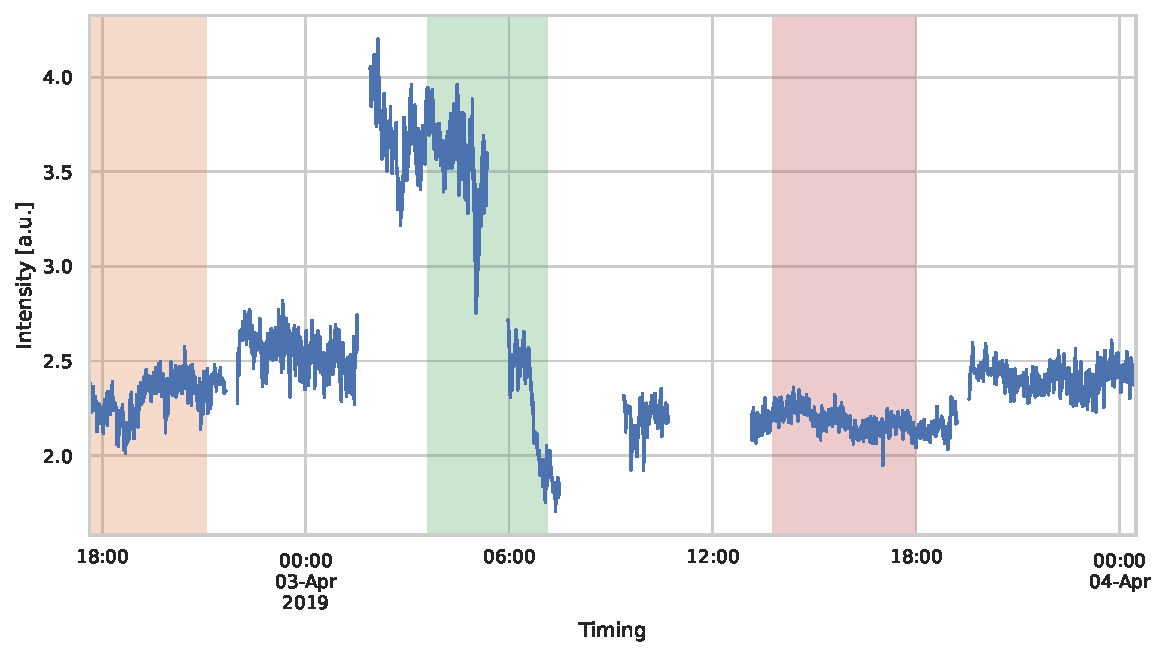
\includegraphics[width=1\linewidth]{images/gmd_grir.pdf}
    \caption{Beam intensity measurements, using the \gls{GMD} over the time period $T=\qty{30}{hour}$, with data window-averaged at \qty{1}{min} intervals. The fluctuations in intensity can be observed, an intrinsic property of the \gls{SASE} process. Other notable observations are the long-term drifts in intensity, and the beam interruptions (no recorded values). The orange, green and red spans indicate the time periods used for other analyses.}
    \label{fig:gmd-intensity}
\end{figure}

We test with two datasets, measured with different light sources: \gls{WSe2} measured with a pulsed laser, and \gls{GrIr} measured with an \gls{FEL}. As seen from the theoretical standing, the statistics from a laser source should be explainable using a homogenous poisson point process, and temporally they should follow a Poisson distribution.
Whereas, the \gls{FEL} source has intensity fluctuations and the expectation is that the statistics should be over-dispersed. Since the intensity variations are themselves random, the cox process is an appropriate model.

Important to note is that the point process is temporally defined and not spatially, meaning that the data points should not be distributed with poisson statistics in space. The data points are not independent in space, as the photoelectrons are ejected from the same material and are correlated. Otherwise, there would be little point to do \gls{PES}.
However, due to sparse data, it becomes necessary to look at small regions, hoping the nearby points are similar enough to not affect the statistics.

The ideal situation would be specially designed experiment that exhibits no spatial correlations and with long enough acquisition time to get a good estimate of the statistics at different time windows.

There are two ways to test the point process. One is to look at the time intervals between events, and the other is to look at the number of events in a fixed time interval. While the light sources give timing information coarser than the electron detection time, the \gls{DLD} detector measures the \gls{TOF} of each electron. Nonetheless, measuring the time intervals between events is not possible due to the dead-time of the detector, after event detection. Hence, we look at the number of events in a fixed time interval.

Specialized tests do exist to directly test for a homogenous Poisson process, hypothesizing complete spatial randomness, Ripley's K-function can be used as a goodness of fit test \cite[Section~2.6.4]{chiuStochasticGeometryIts2013}.

\subsection{Number of events in a fixed time interval}
% \begin{figure}[h]
%     \centering
%     \begin{subfigure}[t]{0.49\linewidth}
%         \centering
%         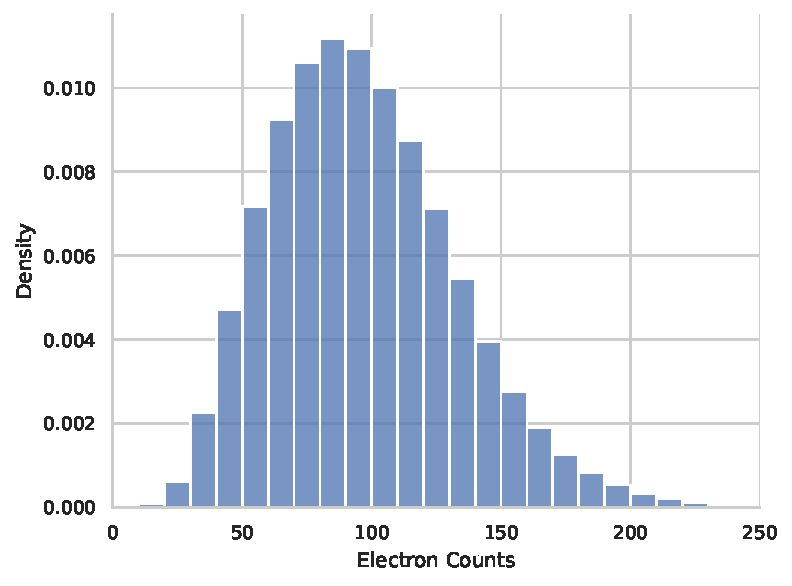
\includegraphics[width=\linewidth]{images/hist_counts_per_train.pdf}
%         \caption{}
%         \label{fig:hist-grir-flash}
%     \end{subfigure}
%     \hfill
%     \begin{subfigure}[t]{0.49\linewidth}
%         \centering
%         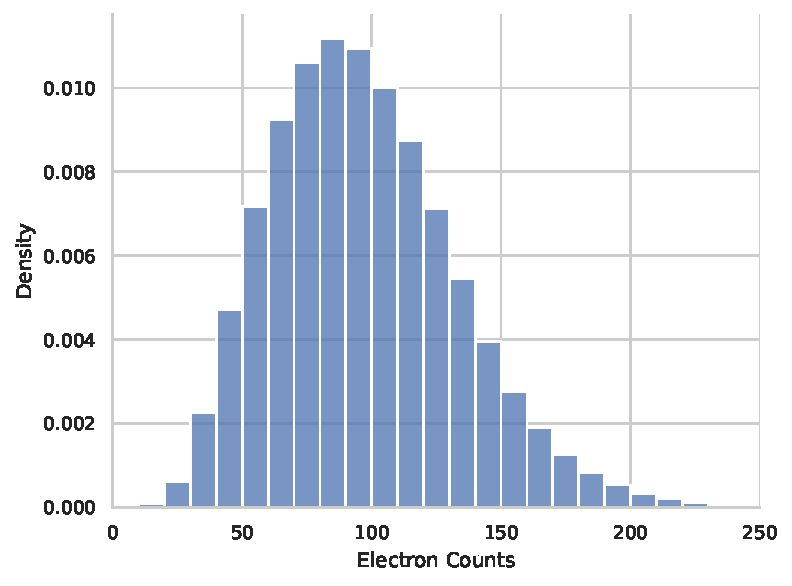
\includegraphics[width=\linewidth]{images/hist_counts_per_train.pdf}
%         \caption{}
%         \label{fig:hist-wse2-laser}
%     \end{subfigure}
%     \caption{}
%     \label{fig:}
% \end{figure}

\begin{figure}
    \centering
    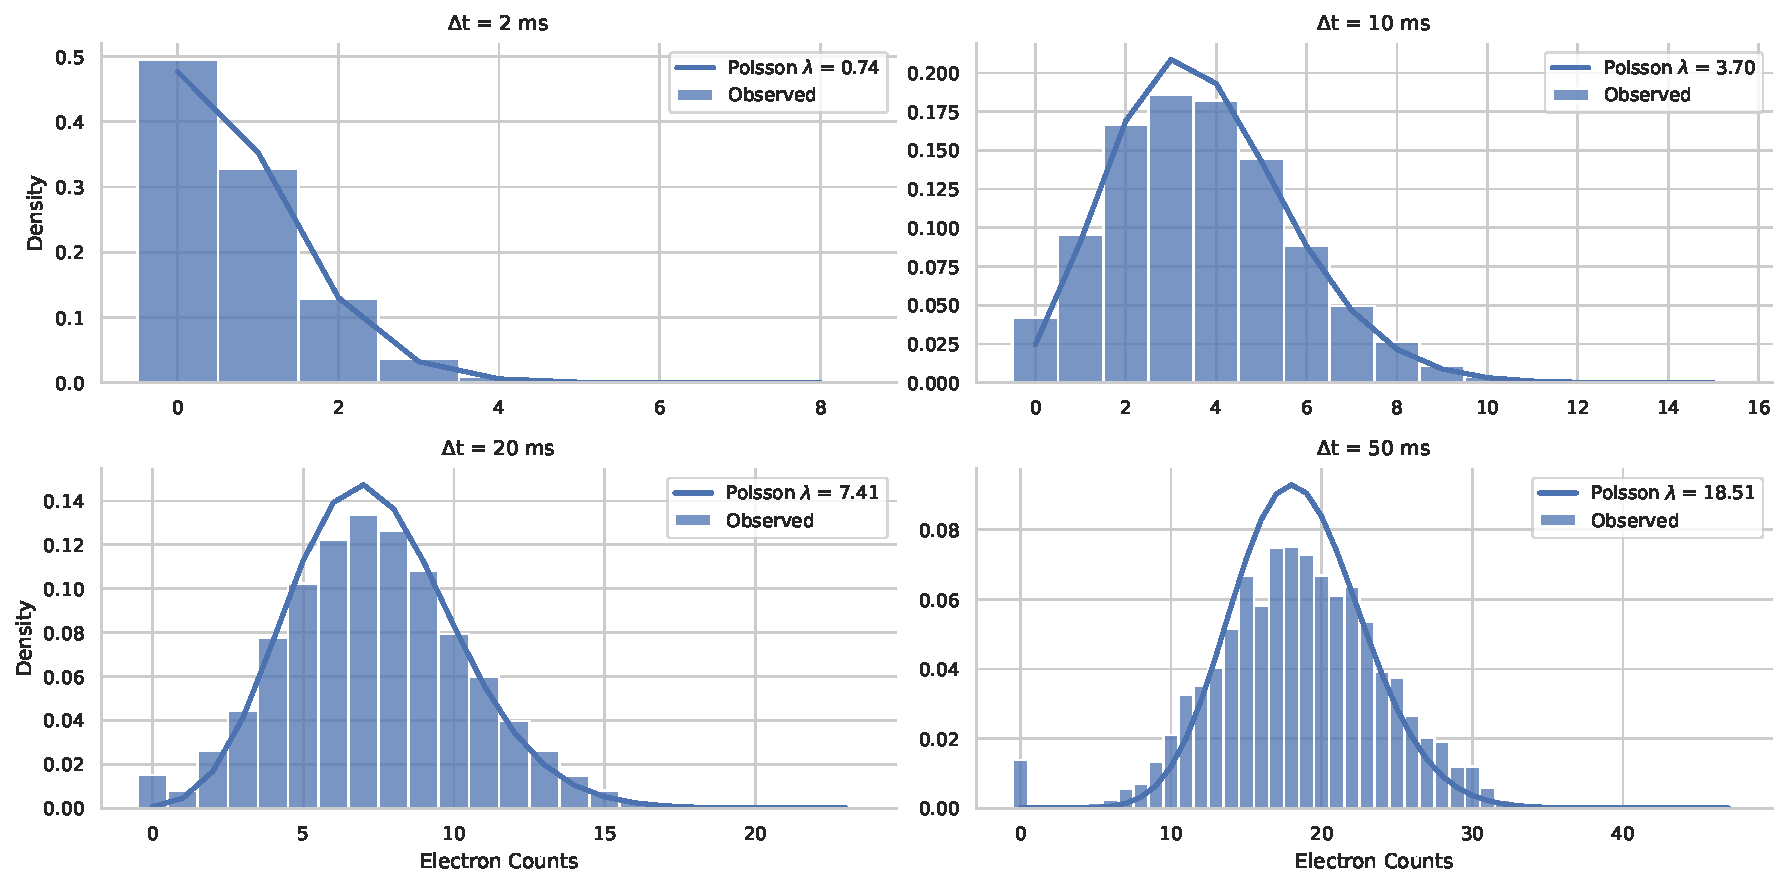
\includegraphics[width=1\linewidth]{images/hist_counts_facetgrid_1_wse2.pdf}
    \caption{Distribution of photoelectron counts at time intervals $\Delta t =$ \qtylist{2;10;20;50}{ms} for a selected volumetric subset of the full \gls{WSe2} dataset. Poisson statistics are observed at smaller time intervals, but as the time window increases ($\Delta t = \qty{50}{ms}$), the data starts to deviate from the Poisson distribution, as spatial correlations become apparent. The total counts in this selected region are $\gls{ncounts}=\num{4.7e4}$ with total observation time $T=\qty{126}{s}$.}
    \label{fig:wse2-stats}
\end{figure}



The Poisson Process can be tested by looking at the number of events in a fixed time interval.

To not induce any spatial correlation effects, that would skew the statistics, we look at a small region in the image space.

Let us look at the dataset using laser first: \gls{WSe2}. \cref{fig:wse2-stats} shows the count distribution at $\Delta t =$ \qtylist{2;10;20;50}{ms}

Testing with small time intervals, we can see that the data follows a Poisson distribution.

However, as we increase the time window, the data starts to deviate from the Poisson distribution. As more events accumulate in the region, the underlying spatial correlations become apparent and start to affect the statistics. The spatial intensity variantions. Then we could describe the process as an inhomogenous poisson process with the spatial intensity determined by the material properties

In practice, it is difficult to test the point process directly. 

As seen in \cref{sec:dld}, special care needs to be taken to draw conclusions using single event data from detector.
We only look at a single sector as we know the two sectors have repeated counts.
Considering the data acquisition scheme of having a pulse and then not, if we try to access the process by taking time intervals, it wouldnt make sense. better would be to look at the data in terms of pulses.
Or we can avoid this issue by looking at time scales above the trainId time scale, where each train comes every 100 ms.
Let us start by looking at the \gls{GrIr} single event data. Ideal would be to look at individual voxels but the counts are way too low so We start by looking at a single dimension, the  axis

To make sure spatial correlations don't impact the statistics, we can look at a 3D patch that is small.

Also interesting to see two pixels at different locations

We hypothesize that the data follows a certain distribution based on theoretical grounding and visualize analysis. Specifically, that data from a laser follows a Poisson distribution and from an \gls{FEL} a \gls{NB} distribution. 

We have seen from \cref{note:poisson-distribution} that the mean and variance of a Poisson distribution are equal. Hence, the simplest way to test if the data follows a Poisson distribution or a \gls{NB} distribution is to compare the sample mean and variance. If the sample mean and variance are equal, then the data follows a Poisson distribution. If the sample mean is greater than the sample variance, then the data follows a \gls{NB} distribution.

For a Poisson distribution, the sample mean is equivalent to the  MLE of the parameter $\lambda$. For a \gls{NB} distribution, the sample mean is not equivalent to the parameter $\lambda$.

Using Chi-Square test, on all points shown in \cref{fig:wse2-stats}, the test shows that the data is better explained by NB. However, on a temporal subset, it's different. This suggests there is some intensity drift in the laser

% The first step in this process is to find the optimal parameters for the Poisson and \gls{NB} distributions. This can be done by fitting the data to the distributions and finding the parameters that minimize the difference between the data and the distribution. The \gls{MLE} is a common method used to estimate the parameters of a distribution. The \gls{MLE} is the value of the parameter that maximizes the likelihood of the data given the distribution. The likelihood is the probability of observing the data given the distribution. The \gls{MLE} is the value of the parameter that makes the data most likely given the distribution.


\begin{figure}[t]
    \centering
    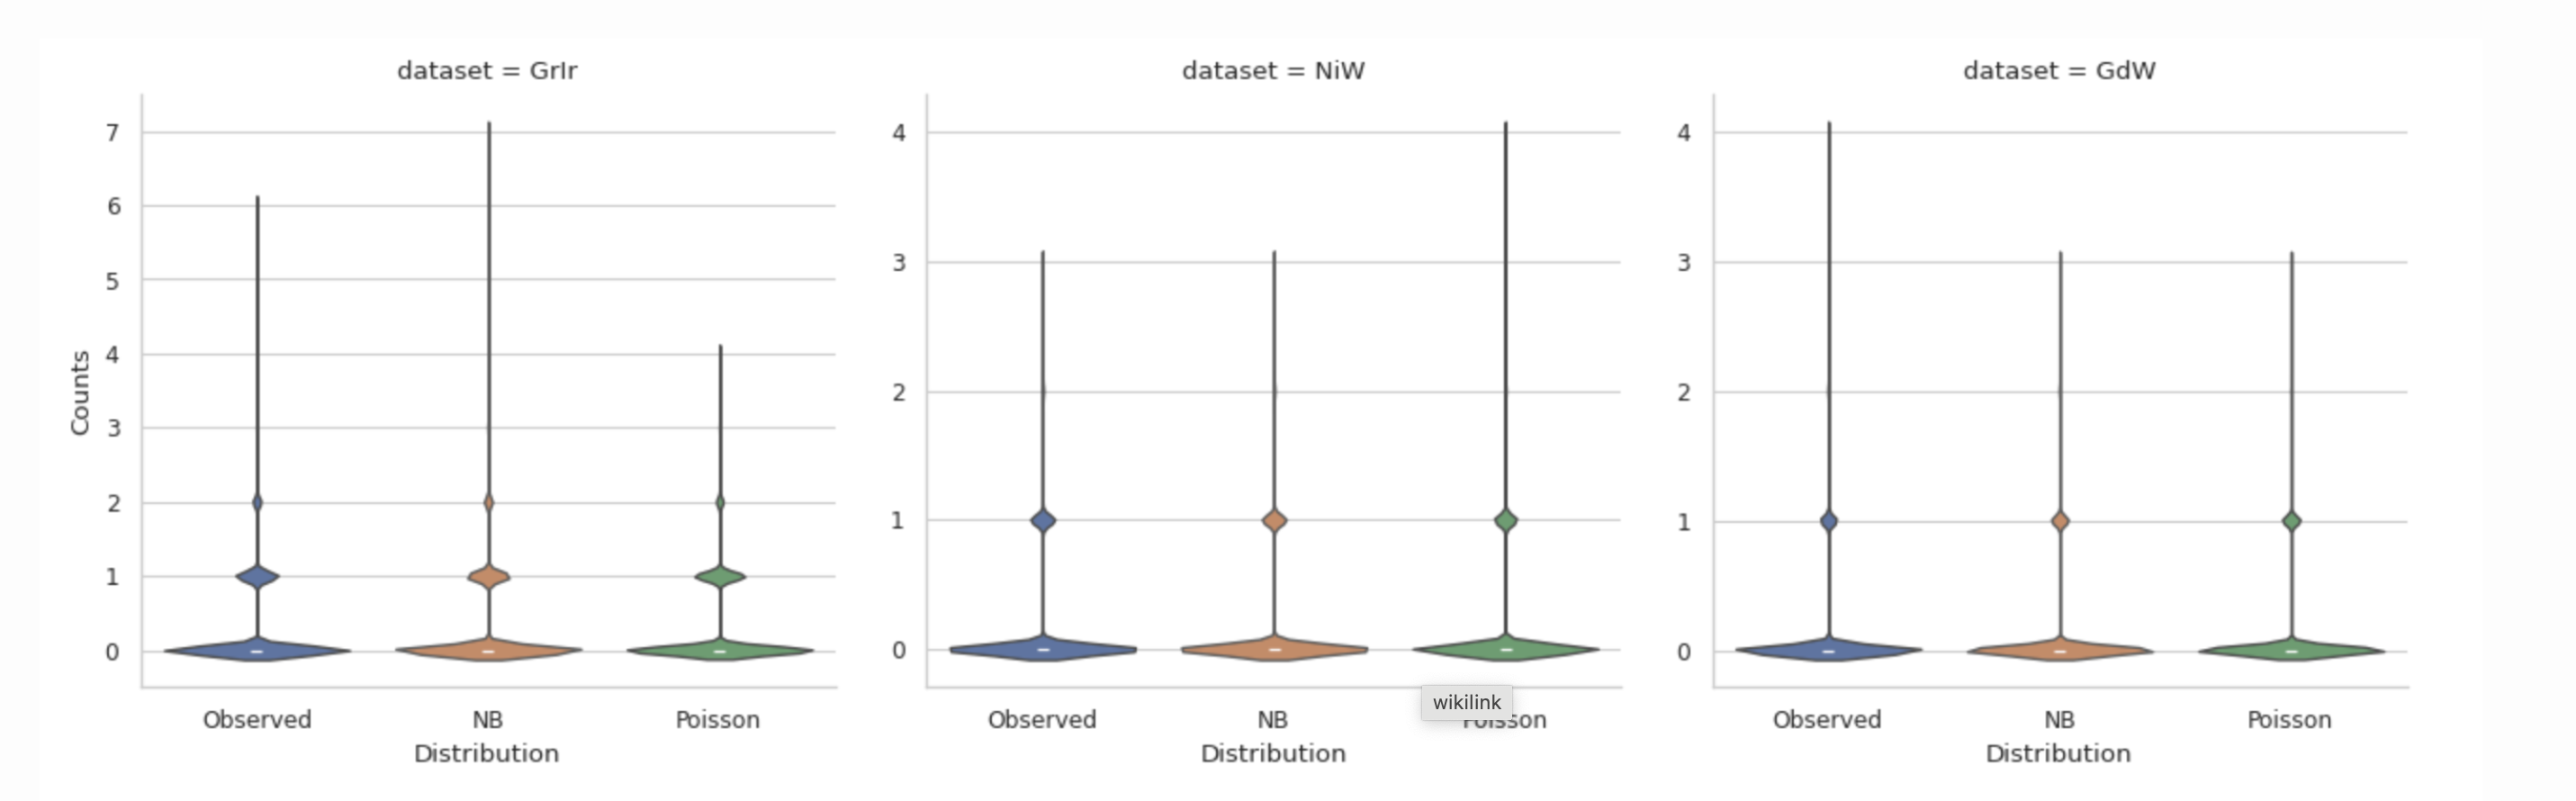
\includegraphics[width=1\linewidth]{images/violin_plots_per_pulse.png}
    \caption{Enter Caption}
\end{figure}

\begin{figure}[htbp]
    \centering
    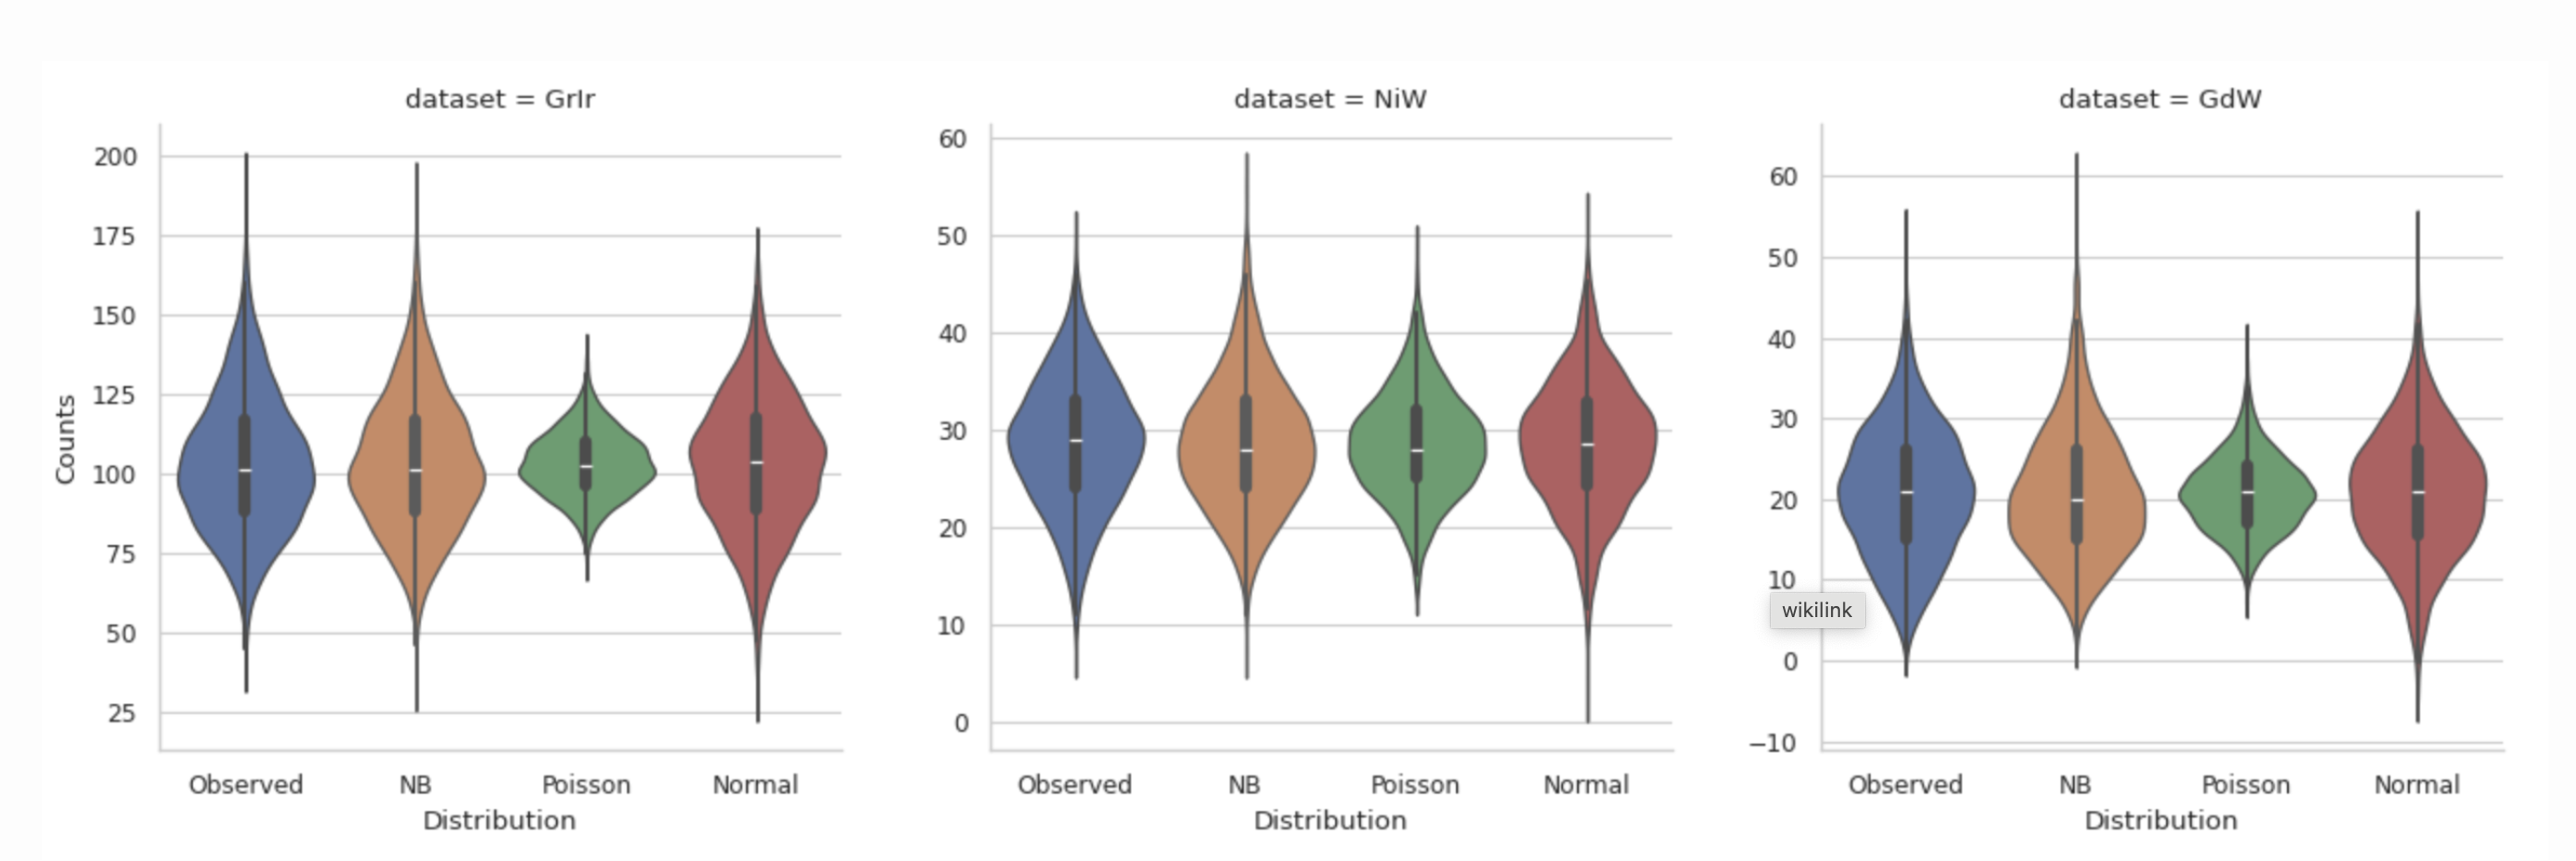
\includegraphics[width=1\linewidth]{images/violinplots_per_train.png}
    \caption{ss}
    \label{s}   
\end{figure}